\documentclass[11pt]{article}
\pagenumbering{gobble}
\usepackage{graphicx}
\setlength\parindent{0pt}

\begin{document}

\section*{Introduction}

Physical activity (PA) has long been established as one of the main contributors to prevent chronic diseases and promote health {\tiny (Kaminsky LA, J Am Hear Assoc. 2014;3(5):e001430; Warburton DER. Curr Opin Cardiol. 2017;32(5):541–56.)}. Evidence shows that lack of PA leads to an increased risk of cardiovascular disease, diabetes, hypertension, osteoporosis, several types of cancer and a higher mortality rate {\tiny (Guthold R. Lancet Glob Heal. 2018;6(10):e1077–86., Lee IM. Lancet. 2012;380(9838):219–29; Shiroma EJ. J Am Heart Assoc. 2014;3(5):7–9.)}. Given the relevant relationship between PA and health, there is an increasing need of accurate and reliable methods of PA assessment on daily life {\tiny (Montoye HJ. Med Sci Sport Exerc. 2000;32(9 Suppl):S439–41.; Plasqui G. Obes Rev. 2013;14(6):451–62; Strath SJ. Circulation. 2013;128(20):2259–79)}. These methods can be either subjective, such as questionnaires, or objective, as direct observation and wearable devices {\tiny (Strath SJ. Circulation. 2013;128(20):2259–79; Troiano RP. Med Sci Sport Exerc. 2005;37(Supplement):S487–9)}. \\

The most commonly used wearable devices to assess PA are accelerometers {\tiny (Strath SJ. Circulation. 2013;128(20):2259–79)}, described as equipments that detect the body movement accelerations in one to three orthogonal planes (anteroposterior, mediolateral, and vertical) {\tiny (Chen KY. Med Sci Sport Exerc. 2005;37(Supplement):S490–500)}. The accelerometers output can be either raw acceleration, usually expressed as gravitational acceleration units (\textit{g}), or activity counts, which are processed data derived from the raw acceleration and are based on manufacturer-specific algorithm {\tiny (Chen KY. Med Sci Sport Exerc. 2005;37(Supplement):S490–500; Bassett  Jr. Med Sci Sport Exerc. 2012;44(1 Suppl 1):S32-8; Troiano RP. Br J Sports Med. 2014;48(13):1019–23)}. In both cases, the accelerometer output needs to be translated into more biologically meaningful information through a calibration process {\tiny (Matthews CE. Med Sci Sport Exerc. 2005;37(11 (Suppl)):S512–22.)}. \\

Currently, most calibration studies use accelerometer output to relate to energy expenditure (EE) and PA intensity levels {\tiny (Migueles JH. Sport Med. 2017;47(9):1821–45; Mendes MA. Gait Posture. 2018;61:98–110)} but they can be also used to estimate biomechanical parameters, such as ground reaction forces (GRF) {\tiny (Neugebauer JM. PLoS One. 2014;9(6):e99023; Fortune E. J Appl Biomech. 2014;30(5):668–74)}, to evaluate standing balance	{\tiny (Mayagoitia RE. Gait Posture. 2002;16(1):55–9)}, to detect the type of PA being performed {\tiny (Bonomi AG. Med Sci Sport Exerc. 2009;41(9):1770–7; Zhang S. Med Sci Sport Exerc. 2012;44(11):2228–34)}, among others. Apart from the standard measure against which the accelerometer output needs to be compared	, calibration studies must carefully define the sample characteristics, PA protocols and statistical approaches, as these aspects can greatly influence the study internal and external validity {\tiny (Bassett  Jr. Med Sci Sport Exerc. 2012;44(1 Suppl 1):S32-8.; Welk GJ. Med Sci Sport Exerc. 2005;37(Supplement):S501–11)}. This led to the emergence of several different calibration studies in the literature with distinct methods to predict a given outcome variable {\tiny (Mendes MA. Gait Posture. 2018;61:98–110, Matthews. Med Sci Sports Exerc. 2018 Jun 21.)}. \\

This current review aims to describe the current literature regarding the use of accelerometers to measure EE, classify physical activity intensities and estimate GRF, as well as issues about calibration and validation studies of these wearable monitors. 

\section*{Accelerometers}

As said before, accelerometers are wearable devices used to measure PA related variables {\tiny (Chen KY. Med Sci Sport Exerc. 2005;37(Supplement):S490–500.)}. The first portable accelerometer was developed in the 1980s {\tiny (Wong TC. IEEE Trans Biomed Eng. 1981;28(6):467–71., Montoye HJ. Med Sci Sport Exerc. 1983;15(5):403–7.)} and with the many technological advances since then, the use of such devices in research is ever growing, with a major increase in the number of published articles mentioning PA or exercise and accelerometers since the early 2000s (Figure \ref{art_year}).

\begin{figure}[h!]
	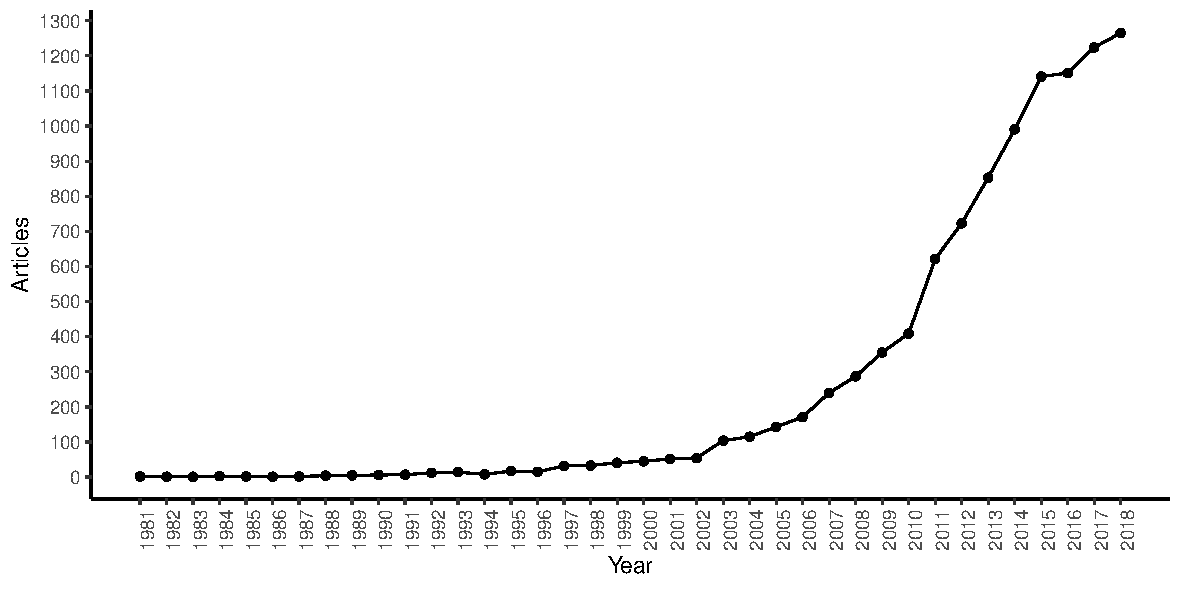
\includegraphics[width=\linewidth]{../figs/fig1.tiff}
	\caption{Articles published by year with search terms "exercise or physical activity" and "accelerometer or accelerometry", Scopus.com, accessed 15 April 2019.}
	\label{art_year}
\end{figure}

From a technical standpoint, the working principle of most accelerometers is based on a sensing element, the seismic mass, and a piezoelectric element. When this system suffers an acceleration, the seismic mass causes a deformation in the piezoelectrical element, generating an output voltage signal proportional to the applied acceleration {\tiny (Chen KY. Med Sci Sport Exerc. 2005;37(Supplement):S490–500., Yang CC, Hsu YL. Sensors. 2010;10(8):7772–88.)}. The rate by which this data is acquired is determined by the sampling frequency of the device, making it responsive not only to the acceleration intensity, but to its frequency {\tiny (Mathie MJ. Physiol Meas. 2004;25(2):R1–20.)}. The signal is then filtered and processed before being digitally stored by the equipment {\tiny (Chen KY. Med Sci Sport Exerc. 2005;37(Supplement):S490–500)}. \\

As an objective method to measure PA, accelerometers offer some advantages over subjective methods, such as questionnaires and PA diaries. They are capable of long data collection with low subject burden {\tiny (Chen KY. Med Sci Sport Exerc. 2012;44(1 Suppl 1):S13-23; Strath SJ. Circulation. 2013;128(20):2259–79)}, are more accurate than questionnaires to measure PA and sedentary behaviour {\tiny (Celis-Morales CA. PLoS One. 2012;7(5); Matthews CE. Med Sci Sport Exerc. 2018;50(2):266–76)} and can measure the full spectrum of daily activities, providing detailed intensity, frequency and duration data {\tiny (Matthews CE. Med Sci Sport Exerc. 2018;50(2):266–76.; Strath SJ. Circulation. 2013;128(20):2259–79)}. \\

On the other hand, accelerometer devices also present some weaknesses. They cannot account for some activities, such as cycling, climbing stairs, weight-lifting and upper-body activities when worn at hip or lower back {\tiny (Strath SJ. Circulation. 2013;128(20):2259–79.)}. Different manufacturers have distinct algorithms to compute activity counts, making these data not comparable between devices {\tiny (Plasqui G. Obes Rev. 2013;14(6):451–62.)}. There is still no consensus on where to place accelerometers on the body, and how to process the data {\tiny (Troiano RP. Br J Sports Med. 2014;48(13):1019–23.)}, and therefore researchers have a great number os methodological decisions to make, such as select the body placement, sampling frequency, epoch length and cut-point or algorithm or equation to use {\tiny (Migueles JH. Sport Med. 2017;47(9):1821–45.)}. \\

\end{document}